\documentclass[11pt]{article}

\usepackage[utf8]{inputenc}
\usepackage[T1]{fontenc}
\usepackage{lmodern}
\usepackage{microtype}
\DisableLigatures[?,!,`,']{encoding = *, family = tt* }
\usepackage{upquote}
\usepackage[margin=1in]{geometry}
\usepackage{graphicx}
\usepackage{booktabs}
\usepackage{array}
\usepackage{amsmath}
\usepackage{amssymb}
\usepackage{amsthm}
\usepackage[hidelinks]{hyperref}
\usepackage{caption}
\usepackage{float}
\captionsetup{font=small,labelfont=bf}

\newtheorem{proposition}{Proposition}
\newtheorem{conjecture}{Conjecture}
\newtheorem{lemma}{Lemma}
\newtheorem{corollary}{Corollary}
\renewcommand{\theta}{\vartheta}
\newcommand{\gap}{\Delta}
\newcommand{\g}[1]{\texttt{#1}}

\title{Maximum Contextuality Gap up to Eleven Vertices\\and Ramsey Structure in the Maximizers}
\author{Dan Mu\textcommabelow{s}etoiu\\
\texttt{dan.musetoiu@gmail.com}} % TODO affiliation
\date{September 2026}

\begin{document}

\maketitle

\begin{abstract}
In the exclusivity-graph approach to contextuality, a noncontextuality inequality is a graph $G$, its noncontextual bound is the independence number $\alpha(G)$ and its quantum bound is the Lov\'asz number $\theta(G)$. The absolute gap $\gap(G)=\theta(G)-\alpha(G)$ was recently maximized exhaustively over all connected graphs on eight vertices. We extend the exhaustive search to nine, ten and eleven vertices --- up to $1{,}006{,}700{,}565$ graphs --- and find $\gap_{\max}=2/3$ ($\theta=11/3$), $1/\sqrt2$ ($\theta=3+1/\sqrt2$) and $0.774889$. The billion-graph search runs in hours on a consumer GPU through a certified screen: a feasible point of the dual semidefinite program is an explicit upper bound on $\theta$, and only graphs whose certified bound can beat the record are solved exactly. At eleven vertices the maximizers change character, from dense graphs with $\alpha=3$ to sparse triangle-free graphs with $\alpha=4$. We explain this by a Ramsey-theoretic tension: triangle-free graphs with $\alpha\le k-1$ are the $R(3,k)$-graphs and exist only below $R(3,k)$ vertices, so Ramsey numbers hold $\alpha$ down while $\theta$ grows. At the critical sizes the record graphs are $R(3,k)$-graphs; the triangle-free maximizer on thirteen vertices is the unique $R(3,5)$-critical graph $C_{13}(1,5)$, with $\theta$ in closed form. The complete catalogues of $R(3,k)$-graphs give a ladder of lower bounds on $\gap_{\max}(n)$ up to $n=35$, and we prove $\gap(G)\le\nu(G)\le n/2$, that $c^*=\lim\gap_{\max}(n)/n$ exists with $0.126\le c^*\le1/2$, and hence $\gap_{\max}(R(3,k)-1)=\Omega(k^2/\ln k)$. Code, graph identifiers and certificates are released.
\end{abstract}

\noindent\textbf{Keywords:} quantum contextuality, exclusivity graphs, Lov\'asz theta number, independence number, Ramsey graphs, semidefinite programming, exhaustive graph search

\section{Introduction}

Which exclusivity graphs separate the quantum from the classical bound of a noncontextuality inequality by the largest amount? For eight vertices the answer was found recently by exhaustive search~\cite{tamer2026}. Here we push the search to eleven vertices, over a billion graphs, and find that the answer changes character on the way: the maximizers stop being dense extensions of the eight-vertex record and become sparse, triangle-free graphs of a very specific kind --- Ramsey graphs. The extremal problem, we argue, is governed not only by the semidefinite geometry of the Lov\'asz number but by a Ramsey-theoretic tension between two invariants: the independence number must be kept small, which Ramsey numbers forbid beyond a certain size unless triangles are admitted, while the theta number grows with the number of vertices. The largest gaps occur exactly at the last sizes where a triangle-free graph can still hold its independence number down.

Cabello, Severini and Winter (CSW) showed that any noncontextuality (NC) inequality of the form $\sum_i P(e_i)\le\alpha$ can be encoded by an \emph{exclusivity graph} $G$ whose vertices are the events $e_i$ and whose edges join mutually exclusive events; the maximum of the left-hand side over noncontextual models is the independence number $\alpha(G)$, and its maximum over quantum models is the Lov\'asz theta number $\theta(G)$~\cite{csw2014}. The gap between the two numbers is therefore a graph invariant that measures how contextual an inequality can be. Two natural figures of merit have been studied: the ratio $\theta/\alpha$, used to identify experimentally accessible witnesses~\cite{amselem2012,canas2016} and as a dimension witness~\cite{ray2021}, and the absolute gap $\gap(G)=\theta(G)-\alpha(G)$, whose maximization over all connected graphs on eight vertices was recently carried out by Tamer et al.~\cite{tamer2026}. Their exhaustive search over the $11{,}117$ graphs identified a sparse ten-edge graph, Quad-$C_5$, with $\gap=0.46784$, beating the Wagner graph ($\gap=\sqrt2-1$).

Two questions follow. What are the maximizers for more vertices, and is there structure behind them? Here we answer the first question exhaustively for $n=9,10,11$ and, for the triangle-free class, for $n=12,13$; and we answer the second by exhibiting a Ramsey-theoretic mechanism and by proving what can be proved about it. The central open statement, for which everything from 8 to 35 vertices below is evidence, is:

\begin{quote}
\emph{At $n=R(3,k)-1$, the maximum of $\gap$ over all graphs on $n$ vertices is attained by an $R(3,k)$-critical graph} (Conjecture~\ref{conj}).
\end{quote}
It is verified over all graphs at $n=8$ ($k=4$: Quad-$C_5$ is triangle-free with $\alpha=3$ on $8=R(3,4)-1$ vertices~\cite{tamer2026}) and, in the triangle-free class, at $n=13$ ($k=5$); for the other critical sizes ($17,22,27,35$) we can only report the maximum over the critical family itself.

\paragraph{Contributions.}
\begin{enumerate}
\item \textbf{Exhaustive maxima for $n=9,10,11$.} $\gap_{\max}(9)=2/3$ exactly, $\gap_{\max}(10)=1/\sqrt2$ exactly, $\gap_{\max}(11)=0.774889$ (Section~\ref{sec:results}). The eleven-vertex search covers all $1{,}006{,}700{,}565$ connected graphs and is, to our knowledge, the first exhaustive computation of a Lov\'asz-number extremum at this scale (the existing table of theta numbers~\cite{cabello2013basic,danielsen-db} stops at ten vertices).
\item \textbf{A certified GPU screening method} (Section~\ref{sec:method}): dual-feasible points of the theta SDP, found by numerical optimization in large batches on a consumer GPU, are explicit upper bounds on $\theta$ that eliminate all but a hundred graphs out of $10^9$; the survivors are solved exactly. The distinction between the search (floating point, heuristic) and the certificate (an explicit matrix whose largest eigenvalue bounds $\theta$) is kept throughout, and the method is validated against every known answer ($n\le 10$) with zero misses.
\item \textbf{Ramsey structure in the maximizers} (Section~\ref{sec:ramsey}). At the Ramsey-critical sizes the record graphs are $R(3,k)$-graphs, i.e.\ triangle-free graphs with $\alpha\le k-1$ on fewer than $R(3,k)$ vertices; in between ($n=9,10$) the maximizers keep the previous independence number by admitting triangles. The thirteen-vertex triangle-free maximizer is the unique $R(3,5)$-critical graph $C_{13}(1,5)$, whose theta number has a closed form. Ramsey numbers thus pin $\alpha$ while $\theta$ keeps growing, and $\gap_{\max}(n)$ jumps at $n=R(3,k)-1$. Computing $\theta$ over the complete catalogues of $R(3,k)$-graphs gives a ladder of lower bounds up to $n=35$.
\item \textbf{Growth} (Section~\ref{sec:theory}). $\gap(G)\le\nu(G)\le n/2$ for every graph (Proposition~\ref{prop:nu}); the gap is superadditive, so $c^*=\lim\gap_{\max}(n)/n$ exists and every record graph bounds it from below, $0.126\le c^*\le\tfrac12$ (Proposition~\ref{prop:fekete}); hence $\gap_{\max}(R(3,k)-1)=\Omega(k^2/\ln k)$ (Corollary~\ref{cor:ramsey}).
\end{enumerate}

\section{Preliminaries}\label{sec:prelim}

Throughout, $G=(V,E)$ is a simple graph on $n$ vertices, interpreted as an exclusivity graph. The independence number $\alpha(G)$ is the size of a largest set of pairwise non-adjacent vertices. The Lov\'asz number~\cite{lovasz1979} can be written as the semidefinite program
\begin{equation}\label{eq:theta-primal}
\theta(G)=\max\bigl\{\langle J,X\rangle : \operatorname{tr}X=1,\ X_{ij}=0\ \forall\,ij\in E,\ X\succeq 0\bigr\},
\end{equation}
where $J$ is the all-ones matrix, with the dual
\begin{equation}\label{eq:theta-dual}
\theta(G)=\min\bigl\{\lambda_{\max}(J+Y) : Y=Y^{\mathsf T},\ Y_{ij}=0\ \forall\, ij\notin E,\ Y_{ii}=0\bigr\}.
\end{equation}
The sandwich theorem gives $\alpha(G)\le\theta(G)\le\alpha^*(G)$, where $\alpha^*$ is the fractional packing number~\cite{knuth1994}. In the CSW framework $\alpha(G)$ and $\theta(G)$ are respectively the noncontextual and the quantum maximum of $\sum_{i\in V}P(e_i)$ over all correlation experiments whose exclusivity graph is $G$~\cite{csw2014}; quantum theory violates the NC inequality iff $\theta(G)>\alpha(G)$, which happens iff $G$ contains an induced odd cycle of length at least five or the complement of one~\cite{cabello2013basic}. We study the \emph{absolute contextuality gap}
\begin{equation}
\gap(G)=\theta(G)-\alpha(G),\qquad \gap_{\max}(n)=\max\{\gap(G): G \text{ connected}, |V(G)|=n\}.
\end{equation}
We also write $f(n)$ for the maximum of $\gap$ over \emph{all} graphs on $n$ vertices, connected or not. The two quantities are tied together by the following elementary facts, used repeatedly below.

\begin{lemma}[Universal vertices and connectivity]\label{lem:mono}
Adding a vertex adjacent to all vertices of $G$ changes neither $\theta$ nor $\alpha$. Consequently $f(n-1)\le\gap_{\max}(n)\le f(n)$ and $\gap_{\max}(n+1)\ge\gap_{\max}(n)$.
\end{lemma}
\begin{proof}
Independent sets are unchanged by a universal vertex $v$, so $\alpha$ is unchanged. In~\eqref{eq:theta-primal} the row and column of $v$ must vanish off the diagonal, so $X=\operatorname{diag}(X',s)$ with $\operatorname{tr}X'=1-s$ and $\langle J,X\rangle=(1-s)\theta(G)+s\le\theta(G)$; hence $\theta$ is unchanged. A universal vertex makes any graph connected, so a (possibly disconnected) maximizer for $f(n-1)$ becomes a connected graph on $n$ vertices with the same gap; the other inequality is trivial, and monotonicity follows by adding a universal vertex to a connected maximizer.
\end{proof}
The two sequences therefore have the same growth, and the connected maximizers of Section~\ref{sec:results} are the interesting objects: a disconnected graph never beats its best component with universal vertices added, since $\theta$ and $\alpha$ are additive over disjoint unions~\cite{knuth1994}.

\begin{lemma}[Ramsey pins $\alpha$]\label{lem:ramsey}
Let $R(3,k)$ denote the Ramsey number, and call a triangle-free graph with $\alpha\le k-1$ an $R(3,k)$-graph. For $R(3,k-1)\le n<R(3,k)$, every triangle-free graph on $n$ vertices has $\alpha\ge k-1$, and those with $\alpha=k-1$ are exactly the $R(3,k)$-graphs on $n$ vertices; for $n\ge R(3,k)$ there are none.
\end{lemma}
\begin{proof}
Immediate from the definition of $R(3,k)$ as the least $n$ such that every graph on $n$ vertices contains a triangle or an independent set of size $k$: on $n\ge R(3,k-1)$ vertices a triangle-free graph has $\alpha\ge k-1$, on $n\ge R(3,k)$ it has $\alpha\ge k$.
\end{proof}

The relevant values are $R(3,4)=9$, $R(3,5)=14$, $R(3,6)=18$, $R(3,7)=23$, $R(3,8)=28$, $R(3,9)=36$~\cite{radziszowski}. McKay's catalogues~\cite{mckay-ramsey,goedgebeur2013} list all $R(3,k)$-graphs for every $n$ when $k\le7$, and at the critical sizes $n=R(3,k)-1$ for $k=8,9$; the $(3,5,13)$ and $(3,9,35)$ graphs are unique~\cite{radziszowski}. Both $\theta$ and $\alpha$ are additive over disjoint unions: for $\alpha$ trivially, for $\theta$ through Lov\'asz's formula $\theta(G)=\max\sum_i\langle c,u_i\rangle^2$ over orthonormal representations $\{u_i\}$ (orthogonal on edges) and unit handles $c$~\cite{lovasz1979}: the sum splits over components, each part being at most the component's $\theta$, and the direct sum of optimal representations with handle $(\sqrt{\theta_1}\,c_1\oplus\sqrt{\theta_2}\,c_2)/\sqrt{\theta_1+\theta_2}$ attains $\theta_1+\theta_2$~\cite{knuth1994}. This fact is used several times below.

\section{Exhaustive results}\label{sec:results}

\subsection{All connected graphs, $n\le 11$}

Table~\ref{tab:main} lists the maximizers of $\gap$ over all connected graphs for $n=5,\dots,11$; the values for $n\le 8$ reproduce~\cite{tamer2026} exactly (including the full top-ten ranking for $n=8$, Appendix~\ref{app:n8}). Figure~\ref{fig:winners} draws the record graphs.

\begin{table}[t]
\centering\small
\caption{Maximum contextuality gap over all connected graphs on $n$ vertices, all rows from our own runs (those for $n\le 8$ agree with~\cite{tamer2026}). Graphs are identified by their graph6 string~\cite{nauty}. The maximizers for $n=9,10,11$ are unique up to isomorphism (the runners-up have $\gap=0.618$, $0.667$, $0.755$). The optimal primal matrix $X$ in~\eqref{eq:theta-primal} has rank $r=4$ for every row with $n\ge 8$ (Appendix~\ref{app:cert}).}
\label{tab:main}
\begin{tabular}{rrlrrrrl}
\toprule
$n$ & \#graphs & graph6 & $|E|$ & $\alpha$ & $\theta$ & $\gap_{\max}(n)$ & remarks \\
\midrule
5 & 21 & $C_5$ & 5 & 2 & $\sqrt5$ & $0.236068$ & KCBS pentagon \\
6 & 112 & \g{EUZO} & 8 & 2 & $\sqrt5$ & $0.236068$ & no improvement over $n=5$ \\
7 & 853 & $C_7$ & 7 & 3 & $3.317667$ & $0.317667$ & \cite{tamer2026} \\
8 & 11{,}117 & \g{GCQb\textasciigrave{}o} & 10 & 3 & $3.467844$ & $0.467844$ & Quad-$C_5$~\cite{tamer2026}; $R(3,4)$-graph \\
9 & 261{,}080 & \g{HCRbdO\{} & 15 & 3 & $11/3$ & $\mathbf{2/3}$ & new; $|\mathrm{Aut}|=12$, one triangle \\
10 & 11{,}716{,}571 & \g{ICRb\textasciigrave{}yiu?} & 20 & 3 & $3+1/\sqrt2$ & $\mathbf{1/\sqrt2}$ & new; 4-regular, $|\mathrm{Aut}|=16$ \\
11 & 1{,}006{,}700{,}565 & \g{J?\textasciigrave{}D@pgd?\{?} & 17 & 4 & $4.774889$ & $\mathbf{0.774889}$ & new; triangle-free, $R(3,5)$-graph \\
\bottomrule
\end{tabular}
\end{table}

\begin{figure}[t]
\centering
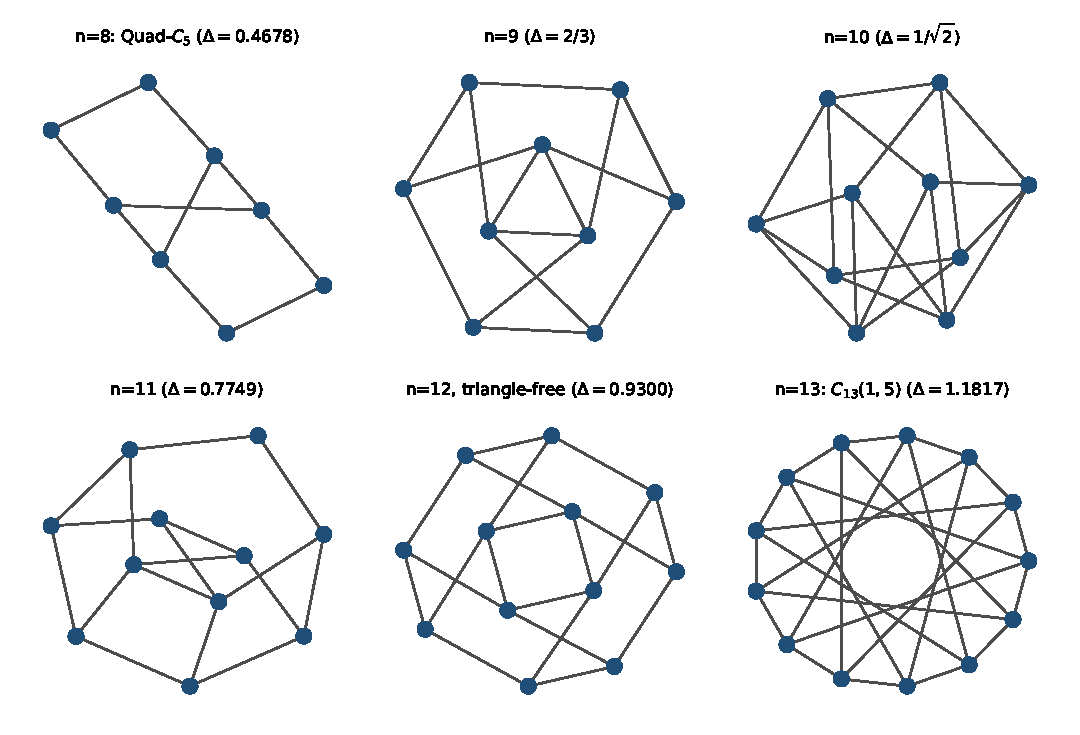
\includegraphics[width=\textwidth]{figures/fig_winners.pdf}
\caption{Record graphs. Top: the exhaustive maximizers for $n=8$ (Quad-$C_5$, \cite{tamer2026}), $n=9$ and $n=10$. Bottom: the exhaustive maximizer for $n=11$, the triangle-free maximizer for $n=12$, and the triangle-free maximizer for $n=13$, which is the circulant Ramsey graph $C_{13}(1,5)$.}
\label{fig:winners}
\end{figure}

\paragraph{$n=9$.} The maximizer \g{HCRbdO\{} has 15 edges, degree sequence $3^6 4^3$, automorphism group of order 12 with vertex orbits of sizes 3 and 6, twelve induced pentagons and a single triangle. Its theta number is $11/3$ to twelve digits (Clarabel with tolerances $10^{-12}$), so $\gap=2/3$ exactly; the optimal $X$ has rank~4. The runner-up (\g{HCrb\textasciigrave{}qi}, 16 edges) is the Wagner graph plus one vertex and has $\theta=2+\varphi=3.618034$, $\varphi$ the golden ratio; it is followed by a large plateau of graphs at exactly Quad-$C_5$'s value $0.467844$ (Quad-$C_5$ plus a vertex that changes neither $\theta$ nor $\alpha$). The maximizer contains neither Quad-$C_5$ nor the Wagner graph as an induced subgraph. Its adjacency spectrum is $\{2+\sqrt2,\,1^{(2)},\,(\sqrt2-1)^{(2)},\,2-\sqrt2,\,-2,\,(-1-\sqrt2)^{(2)}\}$.

\paragraph{$n=10$.} The maximizer \g{ICRb\textasciigrave{}yiu?} is 4-regular with 20 edges, $|\mathrm{Aut}|=16$ (orbits of sizes 2 and 8), sixteen induced pentagons and four triangles, and contains the Wagner graph as an induced subgraph. $\theta=3+1/\sqrt2$ to twelve digits. The runner-up (\g{ICQeR\textasciigrave{}[Mg}, $\gap=0.667155$) contains both Quad-$C_5$ and the $n=9$ maximizer; the ``$n=9$ maximizer plus a vertex'' lineage therefore reaches only second place, as the ``Wagner plus a vertex'' lineage did at $n=9$. The values for $n=9$ and $n=10$ can in principle be read off the table of Cabello, Danielsen, L\'opez-Tarrida and Portillo, who computed $\alpha$, $\theta$ (to four decimals) and $\alpha^*$ for all graphs with $\alpha<\theta$ on up to ten vertices~\cite{cabello2013basic,danielsen-db}; our runs reproduce that table graph-for-graph ($16{,}533$ graphs at $n=9$, $975{,}330$ at $n=10$, $|\theta-\theta_{\rm table}|\le 5.3\times10^{-5}$). The maxima were, however, never reported.

\paragraph{$n=11$.} Here the picture changes. The five best graphs (Table~\ref{tab:n11}) are all triangle-free, have $\alpha=4$ and only 17--19 edges, while the best graph of the dense family that dominated $n\le10$ --- the $n=10$ maximizer plus one vertex, $\gap=0.735505$, which contains Quad-$C_5$, the Wagner graph and the $n=9$ and $n=10$ maximizers as induced subgraphs --- is only sixth. The maximizer \g{J?\textasciigrave{}D@pgd?\{?} has girth 4, degree sequence $2^1 3^8 4^2$, $|\mathrm{Aut}|=2$, eleven induced pentagons and four induced heptagons, and an optimal $X$ of rank $4$. Note that $\gap_{\max}(11)-\gap_{\max}(10)=0.068$ is the smallest increment in the table; the sparse family is only just taking over. Figure~\ref{fig:n11} shows all 100 survivors of the screen: the two families are separated cleanly by edge count, and every graph above the $n=10$ record with fewer than 20 edges is triangle-free.

\begin{figure}[t]
\centering
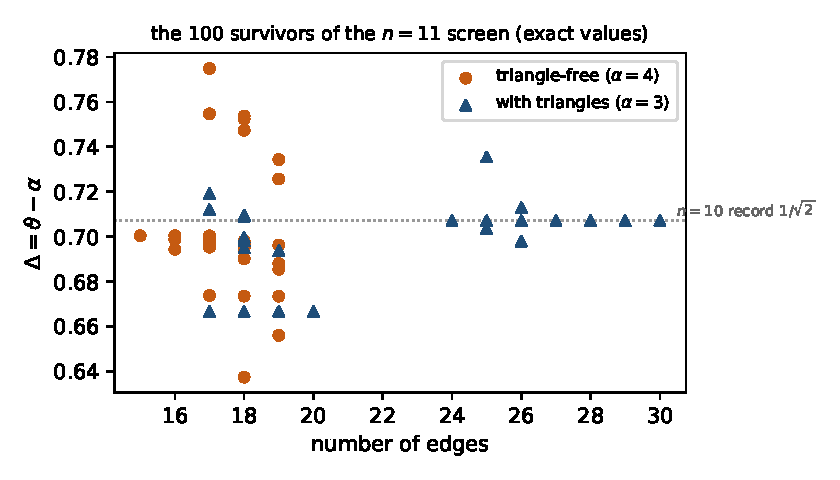
\includegraphics[width=0.75\textwidth]{figures/fig_n11_survivors.pdf}
\caption{The 100 graphs on eleven vertices whose certified bound survived the screen (threshold $1/\sqrt2$), with their exact gaps: the sparse triangle-free family ($\alpha=4$) and the dense family ($\alpha=3$, built around the ten-vertex maximizer).}
\label{fig:n11}
\end{figure}

\begin{table}[t]
\centering\small
\caption{The ten largest gaps among all $1{,}006{,}700{,}565$ connected graphs on eleven vertices. ``tf'' = triangle-free.}
\label{tab:n11}
\begin{tabular}{rlrrrrl}
\toprule
rank & graph6 & $|E|$ & $\alpha$ & $\theta$ & $\gap$ & remarks \\
\midrule
1 & \g{J?\textasciigrave{}D@pgd?\{?} & 17 & 4 & 4.774889 & 0.774889 & tf, $R(3,5)$-graph \\
2 & \g{J?\textasciigrave{}@f?kUDG\_} & 17 & 4 & 4.754686 & 0.754686 & tf \\
3 & \g{J?\textasciigrave{}@f@WFTH?} & 18 & 4 & 4.753664 & 0.753664 & tf, contains Wagner \\
4 & \g{J?\textasciigrave{}FBQoFCi?} & 18 & 4 & 4.752419 & 0.752419 & tf \\
5 & \g{J?\textasciigrave{}@f@Wl?y?} & 18 & 4 & 4.747377 & 0.747377 & tf, contains Quad-$C_5$ \\
6 & \g{JCRbeo\{ifI?} & 25 & 3 & 3.735505 & 0.735505 & $n{=}10$ maximizer $+$ vertex \\
7 & \g{J?\textasciigrave{}FAqSFf\_?} & 19 & 4 & 4.734338 & 0.734338 & tf \\
8 & \g{J?\textasciigrave{}FAosFdI?} & 19 & 4 & 4.725688 & 0.725688 & tf \\
9 & \g{J?\textasciigrave{}DD\textasciigrave{}gD\textasciigrave{}s?} & 17 & 4 & 4.719179 & 0.719179 & tf \\
10 & \g{JCRbeo\{ifM?} & 26 & 3 & 3.712900 & 0.712900 & dense family \\
\bottomrule
\end{tabular}
\end{table}

\paragraph{Gap versus ratio.} The maximizer of the ratio $\theta/\alpha$ is a different graph from the gap maximizer at $n=8,10,11$ (at $n=10$ it is \g{IUZurzmmo} with $\alpha=2$, $\theta=5/2$; at $n=11$ the dense graph in row~6 of Table~\ref{tab:n11}); only at $n=9$ do the two coincide.

\subsection{Triangle-free graphs, $n=12,13,14$}

Motivated by the $n=11$ result we searched exhaustively over connected triangle-free graphs, generated with \texttt{geng -t}~\cite{nauty}: $90{,}842$ graphs for $n=11$ (recovering the global top six), $1{,}144{,}061$ for $n=12$, $19{,}425{,}052$ for $n=13$ and $445{,}781{,}050$ for $n=14$ (6.1 hours on the GPU). The maxima for $n=12,13$ are
\begin{align*}
\gap_{\max}^{\rm tf}(12)&=0.930021\quad(\theta=4.930021,\ \alpha=4,\ 20\text{ edges},\ \g{K?\textasciigrave{}DA\textasciigrave{}gd?\{Dg},\ |\mathrm{Aut}|=8,\ \operatorname{rank}X=5),\\
\gap_{\max}^{\rm tf}(13)&=1.181737\quad(\theta=5.181737,\ \alpha=4,\ 26\text{ edges},\ \g{L?\textasciigrave{}DE\textasciigrave{}gl@YJODg}).
\end{align*}
At $n=13$ the maximizer is isolated: a second exhaustive pass over the class with threshold $0.80$ shows that the next best connected triangle-free graph on 13 vertices has $\gap=0.854480$ ($\theta=5.854480$, $\alpha=5$, 19 edges, \g{L?AAD?oFAgDOAw}); it is also the best connected graph with $\alpha=5$ in the $R(3,6)$ catalogue on 13 vertices, all $275{,}086$ members of which we solved exactly.
The maximizer is 4-regular with $|\mathrm{Aut}|=52$ and is isomorphic to the circulant graph $C_{13}(1,5)$, the unique $(3,5)$-Ramsey-critical graph~\cite{radziszowski}. At $n=14$, the first size at which triangle-free graphs must have $\alpha\ge5$, the exhaustive maximum drops to
\[
\gap_{\max}^{\rm tf}(14)=1.072373\quad(\theta=6.072373,\ \alpha=5,\ 24\text{ edges},\ \g{M?AA@agwAg@WM\_Dc?}),
\]
attained by an $R(3,6)$-graph --- the best connected graph of the $R(3,6)$ catalogue on 14 vertices (Table~\ref{tab:ramsey}) --- and all $12{,}764$ triangle-free graphs on 14 vertices with certified bound above $1.0$ have $\alpha=5$. This is the drop predicted in Section~\ref{sec:ramsey}, now established exhaustively rather than only within the catalogue.

\section{The Ramsey structure of the maximizers}\label{sec:ramsey}

\subsection{The record graphs at the critical sizes are $R(3,k)$-graphs}

For readers less used to Ramsey numbers, the mechanism in one paragraph. $R(3,k)$ is the least $n$ such that every graph on $n$ vertices contains a triangle or $k$ pairwise non-adjacent vertices. Read the other way round: a triangle-free graph on $n\ge R(3,k)$ vertices is forced to have $\alpha\ge k$, while on $n=R(3,k)-1$ vertices there still exist triangle-free graphs with $\alpha=k-1$, and these are by definition the $R(3,k)$-graphs (``critical'' when $n=R(3,k)-1$). Since $R(3,4)=9$, $R(3,5)=14$, $R(3,6)=18$, a triangle-free graph can have $\alpha=3$ only up to 8 vertices, $\alpha=4$ only up to 13, $\alpha=5$ only up to 17. For the gap this matters because $\gap=\theta-\alpha$ rewards a small $\alpha$ at fixed $n$, and $\theta$ of a sparse graph keeps growing with $n$; so the best place to be is the last $n$ at which $\alpha$ can still be held at $k-1$.

By Lemma~\ref{lem:ramsey}, a triangle-free graph with $\alpha\le k-1$ is an $R(3,k)$-graph and exists only for $n<R(3,k)$. Checking the record graphs against McKay's catalogues by isomorphism gives:
\begin{itemize}
\item $n=8$: Quad-$C_5$ and the Wagner graph are two of the three $R(3,4)$-graphs on 8 vertices ($R(3,4)=9$).
\item $n=9,10$: no triangle-free graph has $\alpha=3$ any more; the maximizers keep $\alpha=3$ by admitting one, respectively four, triangles.
\item $n=11$: the maximizer is one of the $105$ $R(3,5)$-graphs on 11 vertices; indeed the 105 connected triangle-free graphs with $\alpha\le4$ on 11 vertices are exactly this catalogue.
\item $n=12$: the triangle-free maximizer is one of the $12$ $R(3,5)$-graphs on 12 vertices.
\item $n=13$: the triangle-free maximizer is the unique $R(3,5)$-graph on 13 vertices, $C_{13}(1,5)$.
\end{itemize}
The mechanism is transparent: $\theta$ grows with $n$ (along the record family at least linearly, Section~\ref{sec:theory}), whereas $\alpha$ is bounded below by Ramsey theory and jumps by one at every $n=R(3,k)$. Records are therefore expected just before the jumps, at $n=R(3,k)-1$, and the gap should \emph{decrease} within the triangle-free class right after a jump. Both regime changes we observe sit exactly on Ramsey numbers: at $n=9=R(3,4)$ the triangle-free graphs with $\alpha=3$ disappear and the maximizers switch to graphs with triangles; at $n=14=R(3,5)$ the triangle-free graphs with $\alpha=4$ disappear and the triangle-free maximum drops from $1.18$ to $1.07$. In between, at $n=11$, the growth of $\theta$ has made $\alpha=4$ triangle-free graphs competitive again, and they overtake the dense $\alpha=3$ family.

\subsection{Circulant Ramsey-critical graphs and closed forms}\label{sec:circ}

Two of the Ramsey-critical vertex counts carry circulant critical graphs, and for those the theta number can be computed in closed form. For a vertex-transitive graph the optimal $X$ in~\eqref{eq:theta-primal} can be taken invariant under the automorphism group~\cite{lovasz1979}; for a circulant $C_n(S)$ this reduces the SDP to a linear program over the Fourier coefficients of a symmetric vector $x\in\mathbb R^n$: $\theta=n\sum_j x_j$ maximized subject to $x_0=1/n$, $x_s=0$ for $s\in\pm S$, and $\hat x_k=\sum_j x_j\cos(2\pi jk/n)\ge0$ for all $k$. Its optimum is therefore an algebraic number in the maximal real subfield of $\mathbb Q(\zeta_n)$. When the graph is moreover edge-transitive, the Lov\'asz--Hoffman bound is attained and the value is explicit~\cite{lovasz1979}:
\begin{equation}\label{eq:hoffman}
\theta(G)=\frac{n\,(-\lambda_{\min})}{\lambda_{\max}-\lambda_{\min}}\qquad(G\ \text{edge-transitive}).
\end{equation}

\begin{proposition}\label{prop:circ}
\begin{enumerate}
\item[(i)] The unique $R(3,5)$-critical graph is the circulant $C_{13}(1,5)$; it is edge-transitive, since the multiplier group $\{\pm1,\pm5\}\subset\mathbb Z_{13}^\times$ acts transitively on the connection set $\{\pm1,\pm5\}$ ($5^2\equiv-1$). Its eigenvalues are $\lambda_j=2\cos(2\pi j/13)+2\cos(10\pi j/13)$, so $\lambda_{\max}=4$, $\lambda_{\min}=2\cos(8\pi/13)-2\cos(\pi/13)$ (multiplicity 4) and
\begin{equation}
\theta\bigl(C_{13}(1,5)\bigr)=\frac{13\,(-\lambda_{\min})}{4-\lambda_{\min}}=5.181736625\ldots,\qquad \gap_{\max}^{\rm tf}(13)=\theta-4=1.181736625\ldots
\end{equation}
\item[(ii)] The unique $R(3,9)$-critical graph, on 35 vertices, is Kalbfleisch's circulant $C_{35}(1,7,11,16)$~\cite{kalbfleisch1966}; it is vertex-transitive but not edge-transitive, and $\theta=12.410586\ldots$ is the optimum of the Fourier linear program (the bound~\eqref{eq:hoffman} gives $12.4979$ and is not attained). Hence $\gap_{\max}(35)\ge 4.410586$. % TODO: closed form from the LP's active set
\item[(iii)] There is no circulant $R(3,k)$-critical graph on $R(3,k)-1$ vertices for $k=6,7,8$ ($n=17,22,27$); the circulant $R(3,k)$-graphs that exist on $16$ and $21$ vertices are not the gap maximizers of their families ($1.1648$ vs $1.4654$; $1.9768$ vs $2.1413$).
\end{enumerate}
\end{proposition}
The scan behind (iii) is exhaustive over connection sets of connected circulants (all $2^{\lfloor n/2\rfloor}$ symmetric sets, triangle-freeness, $\alpha$ by clique search on the complement); a disconnected circulant on these vertex counts has isomorphic components and independence number at least twice that of a component, so it cannot be critical. The identifications in (i) and (ii) are by isomorphism test against McKay's catalogues, whose uniqueness statements for $(3,5,13)$ and $(3,9,35)$ are those of~\cite{radziszowski}.

We note explicitly what Section~\ref{sec:ramsey} does and does not establish. It establishes that $\alpha$ of the triangle-free record graphs is dictated by Ramsey numbers (Lemma~\ref{lem:ramsey}), it identifies every computed triangle-free maximizer, and the global maximizers at $n=8$ and $n=11$, with Ramsey graphs, and for the two circulant cases it gives $\theta$ in closed form. It does not provide a theorem singling out the Ramsey-critical graphs: a lower bound on $\theta$ for triangle-free graphs of small independence number, strong enough to show that the critical graphs beat everything else at $n=R(3,k)-1$, is the missing ingredient. The general lower bounds we are aware of (through $\theta(G)\theta(\bar G)\ge n$ and $\chi(G)=O(\sqrt n)$) are of order $\sqrt n$, below $k-1\approx\sqrt{n\log n}$ at $n=R(3,k)-1$, and do not even certify positivity of the gap; what \emph{can} be proved about growth is in Section~\ref{sec:theory}.

\subsection{A ladder of lower bounds up to $n=35$}

Since the $R(3,k)$-graphs are completely catalogued for $k\le 9$~\cite{mckay-ramsey,goedgebeur2013}, and $\alpha=k-1$ on all of them for $n\ge R(3,k-1)$ (Lemma~\ref{lem:ramsey}), the gap over each catalogue requires only $\theta$. Table~\ref{tab:ramsey} gives the maxima; together with Lemma~\ref{lem:mono} they are lower bounds on $\gap_{\max}(n)$ for all larger $n$. Figure~\ref{fig:ladder} summarizes the results.

\begin{table}[t]
\centering\small
\caption{Maximum gap over all $R(3,k)$-graphs on $n$ vertices (McKay's catalogues; $\alpha=k-1$ analytically, $\theta$ by SDP). These are lower bounds on $\gap_{\max}(n)$. For $n=14$ the catalogue maximum is $C_{13}(1,5)$ plus an isolated vertex; the best connected graph is shown.}
\label{tab:ramsey}
\begin{tabular}{rrrrrrl}
\toprule
$k$ & $n$ & \#graphs & $\alpha$ & $\theta_{\max}$ & $\gap$ & best graph (graph6) \\
\midrule
5 & 13 & 1 & 4 & 5.181737 & 1.181737 & $C_{13}(1,5)$ \\
6 & 14 & 263{,}520 & 5 & 6.072373 & 1.072373 & \g{MqGOOH@\_gQ?oGFCJ?} (connected) \\
6 & 15 & 64{,}732 & 5 & 6.250964 & 1.250964 & \g{NoCOWGACGQIKGePIDI?} \\
6 & 16 & 2{,}576 & 5 & 6.465350 & 1.465350 & \g{OoC?Igi\_?E\_eKcRCE@iO[} \\
6 & 17 & 7 & 5 & 6.606664 & 1.606664 & \g{P@oGQA?\textasciigrave{}ACcdCtDYC]Ah?goC} \\
7 & 21 & 1{,}118{,}436 & 6 & 8.141315 & 2.141315 & \g{THoGG?JODHsOADs\_wg?\textasciigrave{}GgSCZ??ig@@D@?GT} \\
7 & 22 & 191 & 6 & 8.398747 & 2.398747 & \g{UsaC?GGC?DccQDCpKEJAOKW\textasciigrave{}Bo?kD\_[\_okHCUR??} \\
8 & 27 & 477{,}142 & 7 & 10.060569 & 3.060569 & (Appendix~\ref{app:g6}) \\
9 & 35 & 1 & 8 & 12.410586 & 4.410586 & the unique $(3,9)$-critical graph \\
\bottomrule
\end{tabular}
\end{table}

\begin{figure}[t]
\centering
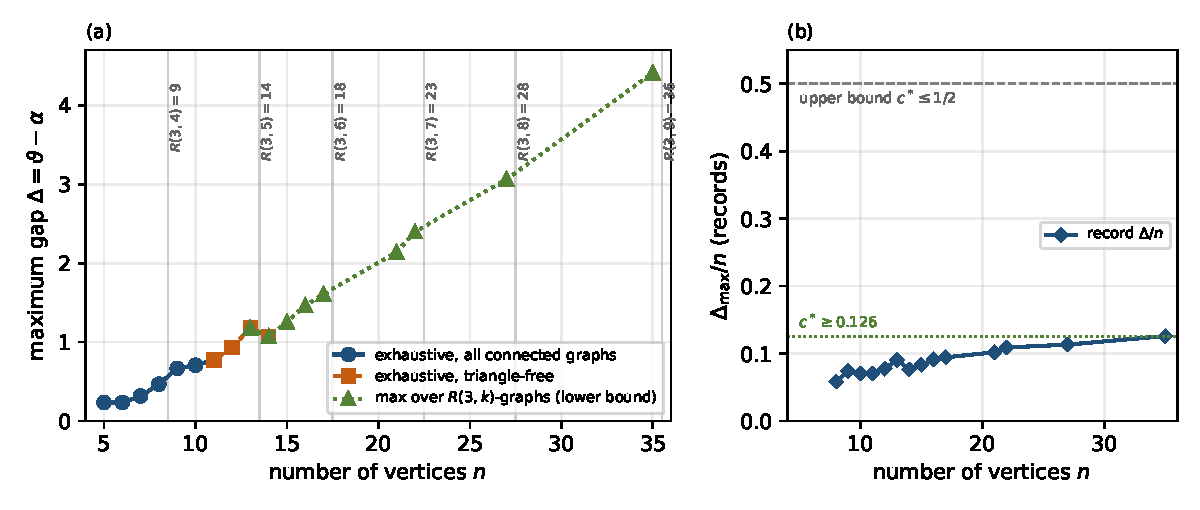
\includegraphics[width=0.85\textwidth]{figures/fig_ladder.pdf}
\caption{(a) Maximum contextuality gap versus number of vertices: exhaustive over all connected graphs ($n\le11$), exhaustive over triangle-free graphs ($n\le14$), and lower bounds from the complete catalogues of $R(3,k)$-graphs. Vertical lines mark the Ramsey numbers $R(3,k)$, where $\alpha$ is forced up by one for triangle-free graphs. (b) Gap per vertex of the record graphs, with the bounds $0.126\le c^*\le\frac12$ of Proposition~\ref{prop:fekete}; the sequence is still increasing at $n=35$.}
\label{fig:ladder}
\end{figure}

The $R(3,6)$-graphs on 13 vertices ($275{,}086$ graphs, for which $\alpha\in\{4,5\}$) confirm the picture from the other side: the single graph with $\alpha=4$ is $C_{13}(1,5)$ with $\gap=1.181737$, and the best of the $275{,}085$ graphs with $\alpha=5$ reaches only $0.930021$ (it is the twelve-vertex triangle-free maximizer plus an isolated vertex).

Within the triangle-free class the maximum gap is \emph{not} monotone: it falls from $1.1817$ at $n=13$ to $1.0724$ at $n=14$ (both exhaustive), exactly as predicted by the jump of $\alpha$ at $R(3,5)=14$, and recovers from $n=15$ on. The global $\gap_{\max}(n)$ is monotone by Lemma~\ref{lem:mono}, but the graphs realizing the monotone extension (a record graph plus universal vertices) are degenerate as witnesses. We are led to:

Call a maximizer of $\gap_{\max}(n)$ \emph{new} if it is not obtained from a maximizer on fewer vertices by adding universal vertices (Lemma~\ref{lem:mono}); the degenerate extensions are never triangle-free, and they carry no information beyond the smaller record.

\begin{conjecture}\label{conj}
(a) For $n=R(3,k)-1$ with $k\ge4$, $\gap_{\max}(n)$ is attained by an $R(3,k)$-critical graph. (b) For $n\ge 11$, every new maximizer is triangle-free, with the least independence number that Ramsey theory allows on $n$ vertices.
\end{conjecture}

We state this as a conjecture with the appropriate caution. The evidence is: the exhaustive result at $n=11$ (the only value where the statement is verified over all graphs), the exhaustive triangle-free results at $n=12,13$, the fact that the mechanism is forced for the two graph invariants separately ($\alpha$ by Ramsey theory, $\theta$ by its growth with $n$ for sparse graphs), and the failure of the ``previous winner plus a vertex'' lineages. The evidence against unrestricted extrapolation is equally clear: for $n=9,10$ the maximizers contain triangles, because no triangle-free graph on nine or more vertices has $\alpha=3$, so an $R(3,4)$-type structure with one or four triangles wins. What the conjecture does \emph{not} say is that Ramsey-critical graphs dominate between the critical vertex counts, nor that every maximizer is triangle-free: at $n=14$ the triangle-free maximum drops (Section~\ref{sec:theory}) and the global maximum is attained only by the degenerate extension of $C_{13}(1,5)$, which has triangles and is not a new maximizer. A brute-force test at $n=12$ would require $1.64\times10^{11}$ graphs; a local search over graphs with triangles at $n=12$ (Section~\ref{sec:discussion}) found nothing above the triangle-free record.

\subsection{What can be proved: a linear upper bound and linear growth}\label{sec:theory}

The Ramsey mechanism pins $\alpha$ from below; the following elementary bound pins $\gap$ from above.

\begin{proposition}\label{prop:nu}
For every graph $G$ on $n$ vertices, $\gap(G)\le\nu(G)\le\lfloor n/2\rfloor$, where $\nu(G)$ is the matching number.
\end{proposition}
\begin{proof}
By the sandwich theorem $\theta(G)\le\bar\chi(G)$, the clique cover number~\cite{knuth1994}. Covering the $2\nu$ vertices of a maximum matching by its $\nu$ edges and the remaining vertices by singletons gives $\bar\chi(G)\le n-\nu$. By the Tutte--Berge formula there is a set $S$ with $n-2\nu=\mathrm{odd}(G-S)-|S|$; one vertex from each odd component of $G-S$ forms an independent set, so $\alpha(G)\ge\mathrm{odd}(G-S)\ge n-2\nu$. Hence $\gap=\theta-\alpha\le(n-\nu)-(n-2\nu)=\nu$.
\end{proof}

The bound is far from tight for small $n$ ($\nu=5$ versus $\gap_{\max}=0.775$ at $n=11$), but it has the right order, and the matching lower bound is elementary: the gap is superadditive, so every record graph is a certificate of linear growth.

\begin{proposition}\label{prop:fekete}
Let $f(n)$ be the maximum of $\gap(G)$ over all graphs (connected or not) on $n$ vertices. Then $f(m+n)\ge f(m)+f(n)$, the limit
\[
c^*=\lim_{n\to\infty}\frac{\gap_{\max}(n)}{n}=\lim_{n\to\infty}\frac{f(n)}{n}=\sup_{G}\frac{\gap(G)}{|V(G)|}
\]
exists, and for every graph $H$ on $h$ vertices and every $n\ge1$,
\[
\gap_{\max}(n)\ \ge\ \Bigl\lfloor\frac{n-1}{h}\Bigr\rfloor\,\gap(H).
\]
In particular, with $H=C_{35}(1,7,11,16)$,
\begin{equation}\label{eq:cstar}
0.1260\ \le\ \frac{\gap(C_{35}(1,7,11,16))}{35}\ \le\ c^*\ \le\ \frac12,\qquad \gap_{\max}(n)\ \ge\ 0.126\,n-4.6\quad(n\ge1).
\end{equation}
\end{proposition}
\begin{proof}
Both $\theta$ and $\alpha$ are additive over disjoint unions~\cite{knuth1994}, so $\gap$ is additive and $f$ is superadditive; $f(n)\le n/2$ by Proposition~\ref{prop:nu}, so Fekete's lemma gives $\lim f(n)/n=\sup f(n)/n$. Adding a vertex adjacent to everything changes neither $\theta$ nor $\alpha$ (proof of Lemma~\ref{lem:mono}) and makes the graph connected, hence $f(n-1)\le\gap_{\max}(n)\le f(n)$ and the two limits coincide. For the explicit bound take $\lfloor (n-1)/h\rfloor$ disjoint copies of $H$ and fill up with universal vertices. The numbers in~\eqref{eq:cstar} are those of Table~\ref{tab:ramsey}.
\end{proof}

Proposition~\ref{prop:fekete} is what Figure~\ref{fig:ladder} shows: the slope of the Ramsey ladder is a lower bound on $c^*$, and each new record graph with a larger ratio $\gap/n$ raises it. Our data give $\gap/n=0.091,\ 0.095,\ 0.109,\ 0.113,\ 0.126$ for the record graphs on $13,17,22,27,35$ vertices, so the best current bound comes from the largest Ramsey-critical graph, and the sequence is still increasing. On the Ramsey side, combining~\eqref{eq:cstar} with Lemma~\ref{lem:mono} and the lower bound $R(3,k)\ge(\tfrac14-o(1))k^2/\ln k$~\cite{bohman-keevash,fgm} gives
\begin{corollary}\label{cor:ramsey}
$\gap_{\max}\bigl(R(3,k)-1\bigr)\ \ge\ 0.126\,R(3,k)-4.8\ =\ \Omega\!\bigl(k^2/\ln k\bigr)$.
\end{corollary}
This explains the growth of the ladder in Table~\ref{tab:ramsey} through the critical vertex counts; it does not explain why the maximizers at those counts are the Ramsey-critical graphs themselves, which remains Conjecture~\ref{conj}. Two heuristics point to a limit strictly between the bounds: for the binomial random graph $G(n,d/n)$, $\theta=\Theta(n/\sqrt d)$~\cite{cojaoghlan2005} while $\alpha\approx(2n/d)\ln d$~\cite{frieze1990}, so sparse random graphs form a second, non-Ramsey family with linear gap; and the upper bound $\nu\le n/2$ is attained only when $\theta=\bar\chi$ and $\alpha=n-2\nu$ simultaneously, which no graph in our tables approaches. Determining $c^*$, and whether the maximizers stay triangle-free, are the natural open problems.

\section{Methods}\label{sec:method}

\subsection{Enumeration and exact computation}
Connected graphs on up to ten vertices were taken from McKay's lists and, for eleven vertices and for the triangle-free classes, generated with \texttt{geng} from \texttt{nauty}~2.8.9~\cite{nauty}, split into resumable \texttt{res/mod} parts. $\alpha$ was computed exactly by enumerating all $2^n$ vertex subsets (bit operations; on the GPU for $n\ge 11$). $\theta$ was computed with the interior-point solver Clarabel~\cite{clarabel} on the primal~\eqref{eq:theta-primal} with tolerances $10^{-9}$ (and $10^{-12}$ for the record graphs), at about $8{,}000$ graphs per second on 20 CPU processes; the full $n=10$ run took 51 minutes.

\subsection{Certified GPU screening for $n=11$}\label{sec:screen}
Exact SDPs for $10^9$ graphs would take several days. Instead we use the dual~\eqref{eq:theta-dual} as a source of certificates and a GPU as a way to search for them. We separate the two roles explicitly.

\paragraph{The certificate.} For any graph $G$ and \emph{any} symmetric matrix $Y$ with $Y_{ij}=0$ whenever $ij\notin E$ (diagonal included), weak duality gives $\theta(G)\le\lambda_{\max}(J+Y)$. Thus a pair $(Y,\lambda)$ with $\lambda\ge\lambda_{\max}(J+Y)$ is a proof that $\theta(G)\le\lambda$, and if moreover $\lambda-\alpha(G)<\gap_{\rm thr}$ then $G$ cannot beat the threshold. Nothing about how $Y$ was found enters this statement. In our implementation $Y$ is a single-precision matrix whose support is enforced exactly by masking, so it is an exactly known rational matrix; the only numerical step in the certificate is the evaluation of $\lambda_{\max}(J+Y)$, done with the batched Jacobi eigensolver of cuSOLVER (through \texttt{torch.linalg.eigh}), which is backward stable. The computed largest eigenvalue of an $n\times n$ symmetric matrix differs from the exact one by at most $c\,n\,u\,\|J+Y\|_2$ ($u=2^{-24}$ in single precision, $c$ a modest constant); in our runs the entries of $Y$ stayed below $7$ in magnitude and $\|J+Y\|_2$ below $15$, so the error is at most $c\cdot10^{-5}$ and $\lambda:=\lambda_{\max}^{\rm computed}+10^{-3}$ is a valid upper bound with a factor of about a hundred to spare. The survivors' final certificates are recomputed in double precision, where the margin is $10^{9}$ times the error, and their $\alpha$ is recomputed independently on the CPU in the exact stage. The run is split into 50 \texttt{res/mod} parts of \texttt{geng}, each producing its own survivor file (in the repository), so it is resumable and auditable part by part; the whole pipeline for $n=11$, including the exact stage, took under three hours of wall time.

\paragraph{The search.} For a batch of $2^{15}$ graphs we optimize $Y$ per graph with 100 Adam steps on the softmax-smoothed largest eigenvalue $\tau\log\sum_i e^{\lambda_i/\tau}$ ($\tau$ annealed from $0.3$ to $0.02$; gradient $V\,\mathrm{diag}(\mathrm{softmax}(\lambda/\tau))\,V^{\mathsf T}$ masked to $E$), using batched single-precision eigendecompositions. Every ten steps the certificate test above is applied and graphs that fail it are removed from the batch; since every intermediate $Y$ is a valid certificate, an early removal is never a false elimination, and a poor optimization can only cost time (a graph that should have been eliminated survives to the exact stage). Survivors are re-solved exactly with Clarabel. With $\gap_{\rm thr}=1/\sqrt2-10^{-6}$ (the $n=10$ record, valid by Lemma~\ref{lem:mono}), the screen processed all $1{,}006{,}700{,}565$ graphs in 2.41~hours on an RTX~2000 Ada (8\,GB) at $0.95$--$1.3\times10^5$ graphs per second, leaving 100 survivors, 51 of which indeed have $\gap\ge1/\sqrt2$.

\paragraph{Validation.} With no threshold, the certified bounds exceed $\theta$ by a median of $0.006$ (max $0.21$) over the $11{,}117$ graphs on eight vertices, and never fall below $\theta$ (Figure~\ref{fig:validation}a). With thresholds $0.60$ at $n=9$ and $0.65$ at $n=10$, the survivors are exactly the two, respectively thirty, graphs known to exceed the threshold (from the exact runs and from~\cite{danielsen-db}), with no misses and no false survivors (Figure~\ref{fig:validation}b).

\begin{figure}[t]
\centering
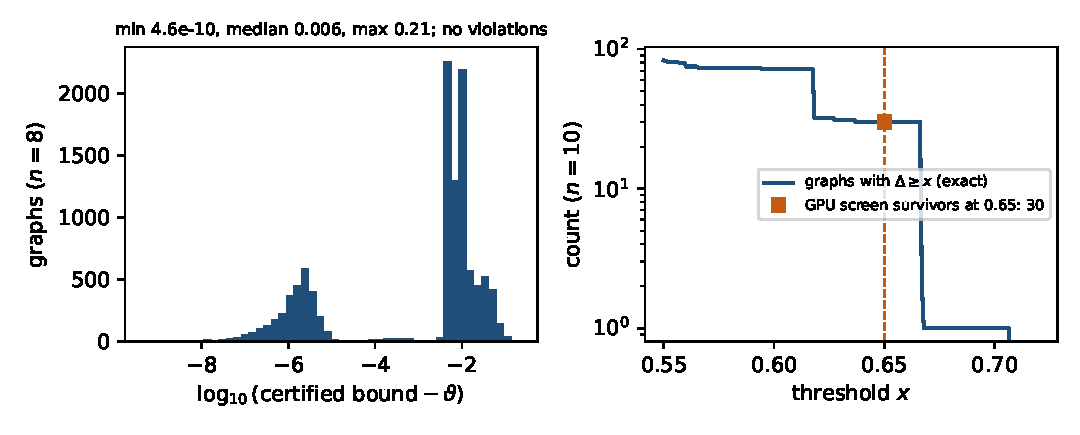
\includegraphics[width=\textwidth]{figures/fig_validation.pdf}
\caption{Validation of the GPU screen. (a) Certified upper bound minus exact $\theta$ for all connected graphs on eight vertices, without pruning. (b) At $n=10$: number of graphs with $\gap\ge x$ from the exact run, and the number of survivors of the screen at threshold $0.65$, which coincides with the exact count.}
\label{fig:validation}
\end{figure}

\subsection{Ramsey catalogues}
For the $R(3,k)$-graphs we used McKay's files \texttt{r35\_13}, \texttt{r36\_14}--\texttt{r36\_17}, \texttt{r37\_21}, \texttt{r37\_22}, \texttt{r38\_27}, \texttt{r39\_35}~\cite{mckay-ramsey}; $\alpha=k-1$ on all of them by Lemma~\ref{lem:ramsey}, and $\theta$ was computed with Clarabel (74 minutes for the $1{,}118{,}436$ graphs on 21 vertices, 88 minutes for the $477{,}142$ graphs on 27 vertices).

\section{Discussion}\label{sec:discussion}

\paragraph{Certificates.} For every record graph we provide an explicit primal feasible matrix $X$ and an explicit dual feasible matrix $Y$ of~\eqref{eq:theta-primal}--\eqref{eq:theta-dual}, recomputed in double precision independently of the solver; they bracket $\theta$ in an interval of width below $10^{-9}$ (Appendix~\ref{app:cert}, Table~\ref{tab:cert}), and the values were reproduced with a second solver (SCS). The exact values $11/3$ and $3+1/\sqrt2$ for $n=9,10$ are thus certified to nine digits; closed forms for the eleven-vertex maximizer and for the triangle-free maximizers on 12 vertices remain to be identified (their minimal polynomials are not obvious from the spectrum, which for $n=11$ contains $2+\sqrt2$ but is otherwise irrational).

\paragraph{Implications for experiments.} From the optimal $X=B^{\mathsf T}B$ one reads off an orthogonal representation of the exclusivity graph in the CSW sense: unit vectors $u_i=b_i/\|b_i\|$, orthogonal for exclusive events, and a state $\psi\propto\sum_i b_i$ with $\sum_i\langle\psi,u_i\rangle^2=\theta(G)$ (Cauchy--Schwarz gives $\ge$, Lov\'asz's theorem gives $\le$). The rank of the maximum-rank optimal $X$ is 4 for all maximizers with $n\le 11$ and for Quad-$C_5$ and Wagner, and 5 for the triangle-free maximizers on 12 and 13 vertices, so all witnesses are realizable with a ququart, respectively a five-level system. We stress that this is an \emph{upper} bound on the minimal dimension: an interior-point solver returns the analytic centre of the optimal face, i.e.\ a maximum-rank optimum, and we make no claim that four (or five) is minimal; settling the minimal dimension requires a separate rank-constrained computation, as done for Quad-$C_5$ in~\cite{tamer2026}. Following~\cite{tamer2026}, the critical visibility under white noise --- the least $v$ for which $v\,\theta+(1-v)\,n/d>\alpha$, i.e.\ $v^*=(\alpha-n/d)/(\theta-n/d)$, smaller being more robust --- is $0.529$ for the $n=9$ maximizer and $0.414$ for the $n=10$ maximizer (with $d=4$), against $0.681$ for Quad-$C_5$ and $0.707$ for the Wagner graph; for the eleven-vertex maximizer $v^*=0.617$ and for $C_{13}(1,5)$ (in $d=5$) $v^*=0.542$. Two conclusions for experiment design follow. First, the new nine- and ten-vertex witnesses are markedly more robust than the eight-vertex ones: the ten-vertex maximizer tolerates $59\%$ white noise, the Wagner graph $29\%$. Second, \emph{a larger gap does not imply a more robust witness}: the eleven-vertex maximizer has a larger gap than the ten-vertex one ($0.775$ vs $0.707$) but needs visibility $0.617$ instead of $0.414$, and $C_{13}(1,5)$, with gap $1.18$, needs $0.542$. The reason is the noise term $n/d$, which grows with $n$ at fixed dimension; the sparse Ramsey-type witnesses pay for their larger gaps with more vertices per dimension. For a given experimental dimension the right figure of merit is $v^*$, and on that count the dense ten-vertex graph is the best witness in our tables. The quoted $v^*$ refer to the realizations we exhibit (dimension $r$); should a lower-dimensional realization of the same graph exist, its noise term $n/d$ would be larger and its $v^*$ worse, so the values above are the best we can certify, not the best possible.

\paragraph{Beyond triangle-free at $n=12$.} A local search over all graphs on twelve vertices, with no triangle-free restriction --- edge additions, deletions and moves with plateau acceptance and random restarts, started from the triangle-free maximizers and from the eleven-vertex records extended by one vertex, with exact $\theta$ and $\alpha$ at every step --- evaluated $1{,}425{,}556$ distinct graphs in 90 minutes. The best gap found was the triangle-free record $0.930021$ itself; the best graph containing a triangle reached $\gap=0.866462$ (one triangle, 21 edges, $\alpha=4$). This is evidence, not proof, for Conjecture~\ref{conj} at $n=12$.

\paragraph{Relation to previous work.} The theta number was introduced to bound the Shannon capacity, $\alpha(G)\le\Theta(G)\le\theta(G)$, with $\theta(C_5)=\sqrt5$ as the founding example~\cite{lovasz1979}; its interplay with independence numbers of graph powers, and through $\theta(G)\theta(\bar G)\ge n$ with Ramsey-type constructions, is surveyed in~\cite{alon}. In that literature $\theta$ is a tool for upper-bounding $\alpha$ of large product graphs; here the object is the \emph{difference} $\theta-\alpha$ of the Ramsey graphs themselves, as a measure of contextuality, and the Ramsey numbers enter through the vertex counts at which $\alpha$ is forced up, not through $\theta$. The graph-enumeration programme of~\cite{cabello2013basic,canas2016} computed $\alpha$, $\theta$ and $\alpha^*$ for all graphs with up to ten vertices and studied ratio maximizers and ``fully contextual'' graphs ($\theta=\alpha^*$); none of the gap maximizers found here is fully contextual (e.g.\ $\alpha^*=13/2$ for $C_{13}(1,5)$), and the two figures of merit select different graphs from $n=8$ on.

\section{Conclusion}
We have pushed the exhaustive maximization of the absolute contextuality gap from eight to eleven vertices, over a billion graphs, with a GPU screening scheme whose every elimination is backed by a dual certificate, and we have found that the answer has a structure: at the Ramsey-critical sizes the record graphs are Ramsey $R(3,k)$-graphs, triangle-free graphs whose independence number is held at $k-1$ by $n<R(3,k)$ while their theta number keeps growing, and in between the maximizers keep the previous independence number by admitting triangles. The thirteen-vertex triangle-free maximizer is the Ramsey graph $C_{13}(1,5)$ itself, with a closed-form theta number, and the catalogues of $R(3,k)$-graphs yield gap records up to 35 vertices. Two questions are left open: whether the maximizer at twelve vertices --- beyond exhaustive reach at $1.6\times10^{11}$ graphs, though within reach of a more aggressive screen --- is still triangle-free (Conjecture~\ref{conj}), and the value of the linear growth constant $c^*=\lim\gap_{\max}(n)/n$, which Proposition~\ref{prop:fekete} confines to $[0.126,\tfrac12]$. For experiments, the new witnesses on nine and ten vertices have exact theta numbers $11/3$ and $3+1/\sqrt2$, realizations in dimension four (from the rank of the SDP optimum; minimality is not claimed), and are given explicitly in the appendix and in the accompanying repository.

\section*{Code and data availability}
All scripts (exact search, GPU screening, Ramsey catalogue processing), the result tables with graph6 identifiers, and the certificates for the record graphs are available at \url{https://github.com/danmusetoiu/contextuality-gap}.

\appendix
\section{Reproduction of the eight-vertex ranking and graph data}\label{app:n8}\label{app:g6}
\begin{table}[H]\centering\small\caption{Top ten connected graphs on eight vertices by $\gap$ (our run, Clarabel), matching Table~II of~\cite{tamer2026} rank for rank.}\label{tab:n8}
\begin{tabular}{rlrrrrrl}\toprule rank & graph6 & $|E|$ & $\alpha$ & $\theta$ & $\gap$ & $\theta/\alpha$ & \\ \midrule
1 & \g{GCQb\textasciigrave{}o} & 10 & 3 & 3.467844 & 0.467844 & 1.155948 & Quad-$C_5$ \\
2 & \g{GCR\textasciigrave{}r\_} & 11 & 3 & 3.438447 & 0.438447 & 1.146149 &  \\
3 & \g{GCrb\textasciigrave{}o} & 12 & 3 & 3.414214 & 0.414214 & 1.138071 & Wagner graph \\
4 & \g{GCRb\textasciigrave{}w} & 12 & 3 & 3.372281 & 0.372281 & 1.124094 &  \\
5 & \g{GCQbdo} & 11 & 3 & 3.372281 & 0.372281 & 1.124094 &  \\
6 & \g{GCp\textasciigrave{}dO} & 10 & 3 & 3.372281 & 0.372281 & 1.124094 &  \\
7 & \g{GQyurg} & 16 & 2 & 2.343146 & 0.343146 & 1.171573 & CHSH-type graph, ratio maximizer \\
8 & \g{GQyurw} & 17 & 2 & 2.338044 & 0.338044 & 1.169022 &  \\
9 & \g{GCpdag} & 11 & 3 & 3.338044 & 0.338044 & 1.112681 &  \\
10 & \g{GUZurw} & 18 & 2 & 2.333333 & 0.333333 & 1.166667 &  \\
\bottomrule\end{tabular}\end{table}

\paragraph{Edge lists of the record graphs} Vertices are $0,\dots,n-1$ in the labelling induced by the graph6 string.
\begin{itemize}
\item Quad-$C_5$ ($n=8$), \g{GCQb\textasciigrave{}o}: 03, 05, 14, 16, 25, 26, 27, 36, 37, 47.
\item $n=9$ maximizer, \g{HCRbdO\{}: 03, 05, 07, 14, 15, 16, 25, 26, 27, 28, 36, 38, 47, 48, 58.
\item $n=10$ maximizer, \g{ICRb\textasciigrave{}yiu?}: 03, 05, 08, 09, 14, 15, 16, 19, 25, 26, 27, 28, 36, 37, 39, 47, 48, 49, 57, 68.
\item $n=11$ maximizer, \g{J?\textasciigrave{}D@pgd?\{?}: (0,4), (0,6), (0,9), (1,5), (1,8), (2,6), (2,7), (2,8), (3,7), (3,9), (3,10), (4,7), (4,8), (4,10), (5,9), (5,10), (6,10).
\item $n=12$ triangle-free maximizer, \g{K?\textasciigrave{}DA\textasciigrave{}gd?\{Dg}: (0,4), (0,6), (0,9), (1,5), (1,7), (1,8), (2,6), (2,8), (2,11), (3,7), (3,9), (3,10), (4,8), (4,10), (4,11), (5,9), (5,10), (5,11), (6,10), (7,11).
\item $C_{13}(1,5)$, \g{L?\textasciigrave{}DE\textasciigrave{}gl@YJODg}: (0,4), (0,6), (0,7), (0,9), (1,5), (1,7), (1,8), (1,11), (2,6), (2,8), (2,9), (2,10), (3,7), (3,9), (3,11), (3,12), (4,8), (4,10), (4,11), (5,9), (5,10), (5,12), (6,11), (6,12), (7,10), (8,12).
\end{itemize}
\paragraph{The $R(3,8)$ record on 27 vertices} graph6 \g{Z@O\textbackslash{}\allowbreak{}MagCADc\textasciigrave{}\allowbreak{}e@O\_\_\textasciigrave{}\allowbreak{}KoHO\_CCHN?\_\allowbreak{}G@DO?d??oCwQ\allowbreak{}i??GTSPK?Dc?\allowbreak{}@YdI?c?}, $|E|=91$, $\theta=10.060569$, $\gap=3.060569$.


\section{Certificates}\label{app:cert}
\begin{table}[h]\centering\small
\caption{Certificates for the record graphs. $[\theta_{\rm lb},\theta_{\rm ub}]$ is the interval certified in double precision by an explicit primal feasible $X$ (trace one, zero on edges, PSD after eigenvalue clipping; the residual on edge entries is below $10^{-9}$) and an explicit dual feasible $Y$ (supported on the edges, $\lambda_{\max}(J+Y)$ recomputed with LAPACK). $r$ is the rank of the maximum-rank optimal $X$ returned by the interior-point solver, hence an upper bound on the minimal dimension of an orthogonal representation attaining $\theta$; $v^*=(\alpha-n/r)/(\theta-n/r)$ is the critical visibility under white noise in dimension $r$. All matrices and the orthogonal representations are in the repository (\texttt{certificates/*.json}).}
\label{tab:cert}
\begin{tabular}{lrrrllrr}\toprule
graph & $n$ & $|E|$ & $\alpha$ & $\theta_{\rm lb}$ & $\theta_{\rm ub}$ & $r$ & $v^*$ \\ \midrule
Quad-$C_5$ ($n=8$) & 8 & 10 & 3 & 3.467843730 & 3.467843730 & 4 & 0.6813 \\
Wagner ($n=8$) & 8 & 12 & 3 & 3.414213562 & 3.414213562 & 4 & 0.7071 \\
$n=9$ maximizer & 9 & 15 & 3 & 3.666666667 & 3.666666667 & 4 & 0.5294 \\
$n=10$ maximizer & 10 & 20 & 3 & 3.707106781 & 3.707106781 & 4 & 0.4142 \\
$n=11$ maximizer & 11 & 17 & 4 & 4.774888533 & 4.774888533 & 4 & 0.6173 \\
$n=11$, rank 2 & 11 & 17 & 4 & 4.754686045 & 4.754686045 & 4 & 0.6235 \\
$n=12$ triangle-free max. & 12 & 20 & 4 & 4.930021465 & 4.930021467 & 5 & 0.6324 \\
$C_{13}(1,5)$ & 13 & 26 & 4 & 5.181736625 & 5.181736625 & 5 & 0.5423 \\
$R(3,6)$ best, $n=16$ & 16 & 35 & 5 & 6.465350297 & 6.465350300 & 5 & 0.5512 \\
$R(3,6)$ best, $n=17$ & 17 & 40 & 5 & 6.606663834 & 6.606663840 & 6 & 0.5742 \\
$R(3,7)$ best, $n=22$ & 22 & 66 & 6 & 8.398747394 & 8.398747399 & 6 & 0.4931 \\
\bottomrule\end{tabular}\end{table}


\begin{thebibliography}{99}
\bibitem{csw2014} A.~Cabello, S.~Severini, and A.~Winter, Graph-theoretic approach to quantum correlations, Phys. Rev. Lett. \textbf{112}, 040401 (2014).
\bibitem{lovasz1979} L.~Lov\'asz, On the Shannon capacity of a graph, IEEE Trans. Inf. Theory \textbf{25}, 1 (1979).
\bibitem{knuth1994} D.~E.~Knuth, The sandwich theorem, Electron. J. Combin. \textbf{1}, A1 (1994).
\bibitem{cabello2013basic} A.~Cabello, L.~E.~Danielsen, A.~J.~L\'opez-Tarrida, and J.~R.~Portillo, Basic exclusivity graphs in quantum correlations, Phys. Rev. A \textbf{88}, 032104 (2013).
\bibitem{danielsen-db} A.~Cabello, L.~E.~Danielsen, A.~J.~L\'opez-Tarrida, and J.~R.~Portillo, Database of quantum graphs, \url{https://www.codetables.de/larsed/quantum_graphs/}.
\bibitem{amselem2012} E.~Amselem, L.~E.~Danielsen, A.~J.~L\'opez-Tarrida, J.~R.~Portillo, M.~Bourennane, and A.~Cabello, Experimental fully contextual correlations, Phys. Rev. Lett. \textbf{108}, 200405 (2012).
\bibitem{canas2016} G.~Ca\~nas, E.~Acu\~na, J.~Cari\~ne, J.~F.~Barra, E.~S.~G\'omez, G.~B.~Xavier, G.~Lima, and A.~Cabello, Experimental demonstration of the connection between quantum contextuality and graph theory, Phys. Rev. A \textbf{94}, 012337 (2016).
\bibitem{ray2021} M.~Ray, N.~G.~Boddu, K.~Bharti, L.-C.~Kwek, and A.~Cabello, Graph-theoretic approach to dimension witnessing, New J. Phys. \textbf{23}, 033006 (2021).
\bibitem{tamer2026} U.~Tamer, \"O.~E.~M\"ustecapl{\i}o\u{g}lu, A.~Dizdar, and Z.~Gedik, The Quad-$C_5$ graph: maximum contextuality gap on eight vertices, arXiv:2605.12828 (2026).
\bibitem{muller2026} A.~Muller and M.~Saniga, Automated search for highly contextual Kochen--Specker proofs, arXiv:2609.19862 (2026).
\bibitem{kcbs2008} A.~A.~Klyachko, M.~A.~Can, S.~Binicio\u{g}lu, and A.~S.~Shumovsky, Simple test for hidden variables in spin-1 systems, Phys. Rev. Lett. \textbf{101}, 020403 (2008).
\bibitem{kalbfleisch1966} J.~G.~Kalbfleisch, Chromatic graphs and Ramsey's theorem, Ph.D. thesis, University of Waterloo (1966).
\bibitem{radziszowski} S.~P.~Radziszowski, Small Ramsey numbers, Electron. J. Combin., Dynamic Survey DS1 (revised regularly).
\bibitem{goedgebeur2013} J.~Goedgebeur and S.~P.~Radziszowski, New computational upper bounds for Ramsey numbers $R(3,k)$, Electron. J. Combin. \textbf{20}, P30 (2013).
\bibitem{mckay-ramsey} B.~D.~McKay, Ramsey graphs, \url{https://users.cecs.anu.edu.au/~bdm/data/ramsey.html}.
\bibitem{nauty} B.~D.~McKay and A.~Piperno, Practical graph isomorphism, II, J. Symbolic Comput. \textbf{60}, 94 (2014).
\bibitem{clarabel} P.~J.~Goulart and Y.~Chen, Clarabel: An interior-point solver for conic programs with quadratic objectives, arXiv:2405.12762 (2024).
\bibitem{bohman-keevash} T.~Bohman and P.~Keevash, Dynamic concentration of the triangle-free process, Random Structures Algorithms \textbf{58}, 221 (2021).
\bibitem{fgm} G.~Fiz Pontiveros, S.~Griffiths, and R.~Morris, The triangle-free process and the Ramsey number $R(3,k)$, Mem. Amer. Math. Soc. \textbf{263}, no.~1274 (2020).
\bibitem{cojaoghlan2005} A.~Coja-Oghlan, The Lov\'asz number of random graphs, Combin. Probab. Comput. \textbf{14}, 439 (2005).
\bibitem{frieze1990} A.~M.~Frieze, On the independence number of random graphs, Discrete Math. \textbf{81}, 171 (1990).
\bibitem{alon} N.~Alon, Lov\'asz, vectors, graphs and codes, in \emph{Building Bridges II: Mathematics of L\'aszl\'o Lov\'asz}, edited by I.~B\'ar\'any, G.~O.~H.~Katona, and A.~Sali, Bolyai Soc. Math. Stud. \textbf{28} (Springer, Berlin, 2019), pp.~1--16.
\end{thebibliography}

\end{document}
